\documentclass{article}

\usepackage{algorithmic}
\usepackage{amsmath}
\usepackage{graphicx}
\usepackage{hyperref}
\usepackage{booktabs}
\usepackage{verbatim}

\begin{document}

\title{SVM Handwriting Classification\\
       Midterm Exam}
\author{Geoffrey Ulman\\
        CSI747}
\date{October 2012}
\maketitle

\section{Primal Soft-Margin SVM}\label{model1}

The primal soft-margin SVM classifier was built using the optimization problem in Equation \ref{svm1}.

\begin{equation}\label{svm1}
\begin{split}
\min 0.5\left( \vec{w} \cdot \vec{w} \right) + C \sum_{i=1}^l \xi_i \\
s.t. \\
\xi_i \ge 0 \\
y_i \left( \left( \vec{x_i} \cdot \vec{w} \right) - b \right) \ge 1 , i = 1,2,...,l
\end{split}
\end{equation}

\subsection{Primal Soft-Margin AMPL Model}

\begin{verbatim}

model;

# lines in file (number of training images)
param l;

# pixels per image (size of training vector)
param n;

# weight on xi penalty coefficient in primal problem
param C;

# output vector (1 or -1)
param y { 1..l };

# input data
param x { 1..l, 1..n };

# hyperplane parameters
var w { 1..n };
var b;

# relaxation allowing for non-separable problems
var xi { 1..l };

minimize obj: 0.5 * ( sum { i in 1..n } w[i]^2 ) +
                C * ( sum { i in 1..l } xi[i] ) ;

s.t. nonneg { i in 1..l }: xi[i] >= 0;

s.t. hplane { i in 1..l }: y[i] *
              ( ( sum { k in 1..n }
                   x[i,k] * w[k] ) - b ) >= 1 - xi[i] ;

option solver loqo;

\end{verbatim}

\subsection{Primal Soft-Margin Results}

\begin{verbatim}

LOQO 6.07: optimal solution (18 QP iterations, 18 evaluations)
primal objective 3.808456385
  dual objective 3.808456358

"option abs_boundtol 2.8429960302606307e-10;"
will change deduced dual values.

w [*] :=
 1 -3.15451e-27   17  1.82133e-10   33 -0.111267      49 -0.0343738
 2  0.118075      18  0.14054       34 -0.301305      50  0.0933198
 3  0.213456      19 -0.0293014     35 -0.442642      51  0.000171579
 4  0.0818948     20 -0.0770882     36 -0.0416026     52 -0.402848
 5  0.0715085     21  0.741797      37  0.0835767     53 -0.0667686
 6  0.0349342     22  0.501937      38  0.0884881     54  0.0430135
 7 -0.0338163     23  0.198454      39 -0.232727      55  0.0195015
 8 -3.15451e-27   24 -0.131832      40 -0.00596055    56 -0.00596055
 9  8.52162e-11   25 -0.111267      41 -0.129117      57  0.0910099
10  0.339545      26 -0.259003      42 -0.631474      58 -0.0155056
11  0.348543      27 -0.217968      43 -0.662013      59  0.0763903
12  0.475353      28 -0.111734      44 -0.151043      60  0.0520377
13  0.000296062   29  0.285148      45  0.0745046     61 -0.240032
14  0.0637961     30  0.328823      46 -0.232932      62  0.037993
15  0.0661811     31  0.179537      47 -0.187038      63  0.148775
16 -3.15451e-27   32 -3.15451e-27   48  0.0581445     64 -3.15451e-27
;

xi [*] :=
  1 3.54215e-10    48 4.28256e-10    95 3.68708e-10   142 3.775e-10
  2 0.463301       49 3.71314e-10    96 3.76266e-10   143 7.32662e-10
  3 1.49441        50 0.0323216      97 0.0920738     144 3.40313e-10
  4 4.08089e-10    51 3.83008e-10    98 0.072318      145 3.31577e-10
  5 4.00877e-10    52 3.89458e-10    99 3.7132e-10    146 4.24756e-10
  6 3.67217e-10    53 3.36558e-10   100 1.84125       147 0.59652
  7 1.20085        54 3.87526e-10   101 1.1496        148 4.18158e-10
  8 3.88911e-10    55 4.30938e-10   102 3.60704e-10   149 3.97591e-10
  9 0.214791       56 0.41072       103 0.00359628    150 4.38972e-10
 10 1.28133e-08    57 4.1869e-10    104 3.91538e-10   151 4.03546e-10
 11 3.94828e-10    58 3.16047e-10   105 2.21851e-09   152 0.565352
 12 3.77228e-10    59 3.90868e-10   106 4.3815e-10    153 0.894454
 13 1.39793e-09    60 2.843e-10     107 4.12031e-10   154 0.375176
 14 3.46076e-10    61 1.6605e-08    108 4.11394e-10   155 3.85445e-10
 15 3.90668e-10    62 3.95981e-10   109 3.07597e-08   156 3.8433e-10
 16 3.89596e-10    63 3.38845e-10   110 0.135305      157 4.00168e-10
 17 3.84253e-10    64 0.263084      111 3.85553e-10   158 4.20697e-10
 18 3.78775e-10    65 7.81376e-10   112 3.71473e-10   159 3.79116e-10
 19 4.17314e-10    66 0.402768      113 4.2554e-10    160 3.89053e-10
 20 3.87605e-10    67 3.44195e-10   114 3.831e-10     161 0.143884
 21 4.04914e-10    68 3.35975e-10   115 3.93818e-10   162 0.199411
 22 3.74905e-10    69 0.662451      116 3.27886e-10   163 4.35077e-10
 23 0.0274426      70 3.82252e-10   117 4.22175e-10   164 4.1439e-10
 24 0.231874       71 3.98174e-10   118 0.140067      165 3.32473e-10
 25 4.19624e-10    72 0.145354      119 0.127478      166 3.72152e-10
 26 1.2731         73 0.945562      120 3.7356e-10    167 6.75207e-10
 27 3.26029e-10    74 0.256505      121 4.11598e-10   168 0.34252
 28 3.88575e-10    75 5.01638e-10   122 3.75389e-10   169 0.575049
 29 8.17445e-10    76 3.87452e-10   123 3.1802e-10    170 4.11112e-10
 30 3.87155e-10    77 1.10393e-07   124 4.17731e-10   171 3.17172e-10
 31 3.61122e-10    78 3.27744e-10   125 4.31632e-10   172 3.99229e-10
 32 7.53563e-10    79 4.31609e-08   126 4.18139e-10   173 3.65298e-10
 33 3.5612e-10     80 3.43132e-10   127 0.911277      174 3.34136e-10
 34 4.35504e-10    81 4.26958e-10   128 3.56167e-10   175 5.7491e-10
 35 3.97985e-09    82 3.73867e-10   129 3.55418e-10   176 0.228682
 36 4.1976e-10     83 0.52189       130 3.69854e-10   177 3.81167e-10
 37 3.87513e-10    84 4.06703e-10   131 3.62618e-10   178 3.75641e-10
 38 1.02411e-08    85 3.83031e-10   132 3.84984e-10   179 0.191379
 39 3.8985e-10     86 3.66646e-10   133 4.17247e-10   180 0.447845
 40 1.84448e-09    87 3.77081e-10   134 2.82501e-09   181 1.42038e-09
 41 4.14366e-10    88 0.846396      135 4.24345e-10   182 3.75385e-10
 42 3.65064e-10    89 1.41052       136 8.34873e-10   183 4.10451e-10
 43 3.91127e-10    90 4.08348e-10   137 4.32896e-10   184 3.636e-10
 44 4.277e-10      91 4.05179e-10   138 3.55676e-09   185 1.45174e-09
 45 4.25439e-10    92 4.19322e-10   139 1.16151       186 4.51322e-10
 46 4.04992e-10    93 4.10816e-10   140 4.31328e-10
 47 0.0204862      94 4.02686e-10   141 3.93777e-10
;

b = 0.0120722

\end{verbatim}

Java was used to parse the AMPL results and the input data files. The hyperplane defined by \(\vec{w}\) and \(b\) was then used to classify the testing data and calculate the misclassification error rate. The following Java snippet calculates the classifier output \(y\) for a set of test data (data parsing and support code omitted for brevity):

\begin{samepage}
\begin{verbatim}

public static double[] calculate_y_predicted_primal(
                            List<TrainingExample> dataListTest,
                            List<TrainingExample> dataListTrain,
                            OutputGenerator out, double[] w, double b )
{
    double[] y_predicted = new double[dataListTest.size( )];

    // iterate over the training examples
    for ( int i = 0; i < dataListTest.size( ); i++ )
    {
        TrainingExample x_i = dataListTest.get( i );

        double sum = 0;
        double[] x = x_i.getInputs( );
        for ( int j = 0 ; j < x.length ; j++ )
        {
            sum += x[j] * w[j];
        }

        y_predicted[i] = sum - b;
    }

    return y_predicted;
}

\end{verbatim}
\end{samepage}

The penalty constant \(C\) was set to \(0.1\) after testing a series of values, running the classifier, and observing the training error. Figure \ref{cvserror} shows the improvement of the testing data error rate as \(C\) approaches \(0.1\).

\begin{figure}\label{cvserror}
\centering
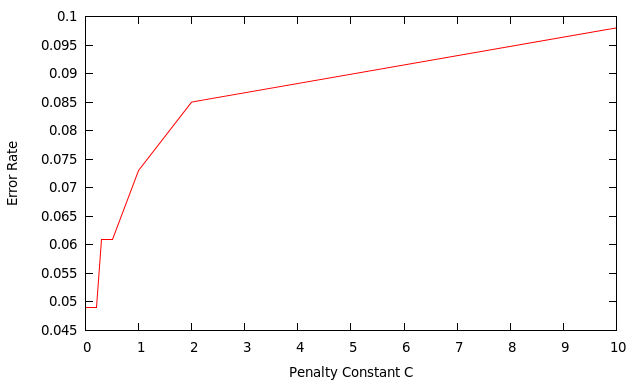
\includegraphics[width=0.9\textwidth]{dual_c_vs_error_rate.png}
\caption{Primal Penality Constant Versus Error Rate}
\end{figure}

\begin{table}\label{table1}
\caption{Primal Soft-Margin Digit 3 vs 6 Error}
\begin{center}
\begin{tabular}{llcc}
\toprule
Data Set & Error & \multicolumn{2}{c}{95\% Confidence Interval} \\
\cmidrule(r){3-4}
& & Lower Bound & Upper Bound \\
\midrule
Training & 0.038 & 0.010 & 0.065 \\
Testing & 0.049 & 0.002 & 0.095 \\
\bottomrule
\end{tabular}
\end{center}
\end{table}

Table \ref{table1} indicates that the primal soft-margin SVM classifier perfectly classified the training data set and acheived a \(0.049\) misclassification error rate for the testing data set for digits ''3`` and ''6``.

\section{Dual Soft-Margin SVM}\label{model2}

The dual soft-margin SVM classifier was built using the optimization problem in Equation \ref{svm2}.

\begin{equation}\label{svm2}
\begin{split}
\max \sum_{i=1}^l \alpha_i - 0.5 \sum_{i,j}^l \alpha_i \alpha_j y_i y_j \left( \vec{x_i} \cdot \vec{x_j} \right) \\
s.t. \\
0 \ge \alpha_i \ge C , i = 1,2,...,l \\
\sum{i=1}^l \alpha_i y_i = 0 , i = 1,2,...,l
\end{split}
\end{equation}

\subsection{Dual Soft-Margin AMPL Model}

\begin{verbatim}

model;

# lines in file (number of training images)
param l;

# pixels per image (size of training vector)
param n;

# weight on xi penalty coefficient in primal problem
param C;

# output vector (1 or -1)
param y { 1..l };

# input data
param x { 1..l, 1..n };

# dual problem variables and simple constraints
var a { 1..l } >= 0, <= C ;

maximize obj: ( sum { i in 1..l } a[i] ) -
                0.5 * sum { i in 1..l, j in 1..l }
                          ( a[i] * a[j] * y[i] * y[j] *
                          sum { k in 1..n } ( x[i,k] * x[j,k] ) ) ;

s.t. const: sum { i in 1..l } a[i] * y[i] = 0 ;

option solver loqo;

\end{verbatim}

\subsection{Dual Soft-Margin Results}

\begin{verbatim}

LOQO 6.07: optimal solution (24 QP iterations, 24 evaluations)
primal objective 3.80845635
  dual objective 3.8084564
a [*] :=
  1 9.08547e-10    48 9.32775e-11    95 7.93618e-11   142 2.44836e-10
  2 0.1            49 9.12306e-10    96 4.20253e-10   143 0.0401223
  3 0.1            50 0.1            97 0.1           144 7.69043e-10
  4 1.2248e-10     51 1.31798e-10    98 0.1           145 1.81561e-09
  5 9.73511e-11    52 1.30999e-10    99 0.0119755     146 1.19908e-10
  6 4.27862e-10    53 2.61964e-09   100 0.1           147 0.1
  7 0.1            54 1.2823e-10    101 0.1           148 2.10874e-10
  8 2.09772e-10    55 8.28051e-11   102 1.58991e-09   149 1.23291e-10
  9 0.1            56 0.1           103 0.0999983     150 9.75451e-11
 10 0.0825943      57 1.39014e-10   104 4.12959e-10   151 1.69916e-10
 11 1.52064e-10    58 7.97273e-10   105 0.0700139     152 0.1
 12 1.1513e-10     59 1.02462e-10   106 1.41395e-10   153 0.1
 13 0.064105       60 4.79618e-08   107 1.2443e-10    154 0.1
 14 3.18092e-10    61 0.090468      108 2.16825e-10   155 1.82193e-10
 15 1.68031e-10    62 1.43344e-10   109 0.0896112     156 5.54399e-10
 16 4.6803e-10     63 2.35787e-09   110 0.1           157 1.47753e-10
 17 5.46372e-10    64 0.1           111 0.0179415     158 3.02381e-10
 18 5.45239e-10    65 0.0437021     112 9.37855e-11   159 2.65331e-10
 19 3.3423e-10     66 0.1           113 1.54081e-10   160 3.81309e-10
 20 1.16503e-10    67 6.13164e-09   114 2.23757e-10   161 0.1
 21 8.35008e-11    68 2.57918e-09   115 2.49166e-10   162 0.1
 22 8.02316e-11    69 0.1           116 3.75511e-09   163 9.7388e-11
 23 0.1            70 4.9684e-10    117 9.24059e-11   164 2.17704e-10
 24 0.1            71 4.38411e-10   118 0.1           165 0.0135987
 25 9.85652e-11    72 0.1           119 0.1           166 5.83863e-10
 26 0.1            73 0.1           120 6.04793e-10   167 0.0325091
 27 1.1187e-09     74 0.1           121 1.17864e-10   168 0.1
 28 0.00971835     75 0.050468      122 1.48579e-10   169 0.1
 29 0.0495885      76 0.0180752     123 7.44134e-09   170 0.0182398
 30 2.73722e-10    77 0.0947431     124 1.73175e-10   171 5.85755e-09
 31 7.17799e-10    78 3.29336e-09   125 1.91625e-10   172 8.09361e-11
 32 0.0255155      79 0.0942866     126 2.17789e-10   173 4.83287e-10
 33 1.56251e-09    80 3.20645e-08   127 0.1           174 8.49808e-10
 34 1.18584e-10    81 1.96128e-10   128 4.13511e-10   175 0.0318319
 35 0.0770716      82 9.77418e-10   129 7.37342e-10   176 0.1
 36 2.19962e-10    83 0.1           130 5.11948e-10   177 4.68524e-10
 37 1.19845e-10    84 1.50151e-10   131 8.73983e-10   178 3.90043e-10
 38 0.0910098      85 1.09665e-10   132 2.72968e-10   179 0.1
 39 1.56061e-10    86 1.0144e-09    133 7.22915e-11   180 0.1
 40 0.0661812      87 1.32879e-09   134 0.0721417     181 0.0625603
 41 1.32986e-10    88 0.1           135 9.82361e-11   182 2.544e-10
 42 5.83862e-10    89 0.1           136 0.0445782     183 1.22333e-10
 43 9.79412e-11    90 1.80474e-10   137 1.97218e-10   184 1.73124e-09
 44 1.8122e-10     91 8.51483e-11   138 0.067866      185 0.0666886
 45 1.19837e-10    92 1.05237e-10   139 0.1           186 1.00778e-10
 46 1.60272e-10    93 1.42097e-10   140 1.73984e-10
 47 0.1            94 0.0178502     141 1.16911e-10
;

\end{verbatim}

The value of \(b\) was calculated for all support vectors (those with \(0 < \alpha_i < C\)) as a check on the correctness of the solution. The table below displays the calculated \(b\) values for each such \(\alpha\). The final \(b\) value used in the classification of the testing data was the average of these \(b\) values.

\begin{verbatim}

#alpha index, alpha value, calculated b
6 0.5531 0.188856798305
8 0.3733 0.188861160199
9 0.0029 0.188871934348
12 0.0531 0.188864376841
18 0.0393 0.188854459866
22 0.0602 0.188871164725
25 0.4170 0.188862548853
27 0.2798 0.188865861802
28 0.5098 0.188865357024
34 0.7256 0.188849350391
37 0.1898 0.188853567449
46 0.1669 0.188858772546
48 0.2942 0.188851064662
52 0.5802 0.188862980571
55 0.7082 0.188853273441
63 0.3538 0.188866929197
68 0.6685 0.188871266426
72 0.8144 0.188867736297
73 0.1018 0.188857462442
77 0.0754 0.188856395052
87 0.0556 0.188872370964
96 0.1804 0.188853107931
97 0.5155 0.188852990917
100 0.4256 0.188855950912
102 0.0825 0.188854038379
104 0.1136 0.188870270977
115 0.5621 0.188873322808
118 0.0967 0.188872624401
126 0.7636 0.188865448670
130 0.1043 0.188856390173
133 0.0968 0.188847704220
138 0.7243 0.188857459050
142 0.0527 0.188860768228
146 0.2022 0.188850473924
151 0.4116 0.188865036435
152 0.8614 0.188865290240
153 0.4057 0.188868509620
160 0.5062 0.188870428611
164 0.6873 0.188869861530
168 0.7740 0.188854538469
169 0.1119 0.188854672264
179 0.1979 0.188858462089
184 0.1469 0.188857771249

\end{verbatim}

Java was used to parse the AMPL results and the input data files above. The hyperplane implied by the primal variable \(\vec{a}\) and the calculated \(b\) was then used to classify the testing data and calculate the misclassification error rate. The following Java snippet calculates the classifier output \(y\) for a set of test data (data parsing and support code omitted for brevity):

\begin{samepage}
\begin{verbatim}

public static double[] calculate_y_predicted( List<TrainingExample> dataListTest,
                                              List<TrainingExample> dataListTrain,
                                              OutputGenerator out, Kernel kernel,
                                              double[] a, double b )
{
    double[] y_predicted = new double[dataListTest.size( )];

    // iterate over the training examples
    for ( int i = 0; i < dataListTest.size( ); i++ )
    {
        TrainingExample x_i = dataListTest.get( i );

        // compute a y_predicted value based on the alpha vector
        // (solution to the dual problem)
        double sum = 0.0;
        for ( int j = 0; j < a.length; j++ )
        {
            TrainingExample x_j = dataListTrain.get( j );
            double y_j = out.getOutput( x_j );
            double a_j = a[j];

            sum += y_j * a_j * kernel.getValue( x_j.getInputs( ), x_i.getInputs( ) );
        }

        y_predicted[i] = sum - b;
    }

    return y_predicted;
}

\end{verbatim}
\end{samepage}

\begin{table}\label{table2}
\caption{Dual Soft-Margin Digit 3 vs 6 Error}
\begin{center}
\begin{tabular}{llcc}
\toprule
Data Set & Error & \multicolumn{2}{c}{95\% Confidence Interval} \\
\cmidrule(r){3-4}
& & Lower Bound & Upper Bound \\
\midrule
Training & 0.038 & 0.010 & 0.065 \\
Testing & 0.049 & 0.002 & 0.095 \\
\bottomrule
\end{tabular}
\end{center}
\end{table}

Table \ref{table2} indicates that the dual soft-margin SVM classifier perfectly classified the training data set and acheived a \(0.049\) misclassification error rate for the testing data set for digits ''3`` and ''6``. This is identical to the results achieved for the primal problem (which makes sense because the formulations should be equivalent). The same penality constant value \(C=0.1\) was the best value for the dual problem as well as the primal problem.

\section{Dual Polynomial SVM}\label{model3}

The dual polynomial SVM classifier was built using the optimization problem in Equation \ref{svm3}.

\begin{equation}\label{svm3}
\begin{split}
\max \sum_{i=1}^l \alpha_i - 0.5 \sum_{i,j}^l \alpha_i \alpha_j y_i y_j \left( \alpha \left( \vec{x_i} \cdot \vec{x_j} \right) + \beta \right)^d \\
s.t. \\
0 \ge \alpha_i \ge C , i = 1,2,...,l \\
\sum{i=1}^l \alpha_i y_i = 0 , i = 1,2,...,l
\end{split}
\end{equation}

\subsection{Dual Polynomial AMPL Model}

\begin{verbatim}

model;

# lines in file (number of training images)
param l;

# pixels per image (size of training vector)
param n;

# weight on xi penalty coefficient in primal problem
param C;

# polynomial machine kernel parameters
param alpha;
param beta;
param delta;

# output vector (1 or -1)
param y { 1..l };

# input data
param x { 1..l, 1..n };

# dual problem variables and simple constraints
var a {1..l} >= 0, <= C;

maximize obj: sum { i in 1..l } a[i] -
              0.5 * sum { i in 1..l, j in 1..l }
                           a[i] * a[j] * y[i] * y[j] * ( alpha * (
                           sum { k in 1..n } x[i,k] * x[j,k] ) + beta ) ^ delta;

s.t. const: sum { i in 1..l } a[i] * y[i] = 0;

option solver loqo;

\end{verbatim}

\subsection{Dual Polynomial Results}

\begin{verbatim}

LOQO 6.07: optimal solution (22 QP iterations, 22 evaluations)
primal objective 2867.882418
  dual objective 2867.882425
a [*] :=
  1   1.02531e-07    48   8.61577e-09    95   2.10839e-08   142   1.48999e-08
  2  98.4474         49   4.61188e-07    96  34.9011        143  27.6442
  3 100              50  30.4183         97  37.7857        144   4.66503
  4   6.5328e-08     51   1.86643e-06    98  10.8704        145   2.7213e-08
  5   1.2032e-07     52   1.11213e-07    99  25.9701        146   1.4305e-08
  6  12.9816         53  97.8993        100 100             147  25.5623
  7  28.3116         54   4.77467e-08   101  23.6605        148   9.86569e-09
  8   6.33472e-08    55   7.64781e-09   102   2.27673e-08   149   1.32595e-08
  9  44.7894         56   8.51246       103   5.24267e-07   150   2.33402e-08
 10  26.3581         57   1.39012e-08   104  10.3686        151   1.542e-08
 11  36.7381         58   4.29743e-07   105  39.3451        152   2.82917
 12   1.07092e-07    59   2.05962e-08   106   4.16072e-07   153 100
 13  74.2736         60 100             107   2.71187e-08   154 100
 14  11.9111         61   8.48449e-08   108   4.24606       155  39.1819
 15   1.82933e-08    62   3.15818e-08   109 100             156   8.86615
 16   1.35129e-07    63  16.6566        110  36.8726        157   3.07667e-08
 17  41.4348         64  63.5389        111  53.4906        158   1.05893e-07
 18  20.8818         65  36.6983        112   7.23013       159   2.16737e-05
 19   4.30859e-06    66 100             113  19.614         160   3.15004e-08
 20   3.23797        67   0.000156624   114  10.0767        161  67.9115
 21   1.43615e-08    68  89.4563        115 100             162   1.16297e-07
 22 100              69 100             116 100             163   8.37258e-09
 23 100              70   2.0411e-08    117   8.08354e-09   164   1.87303e-08
 24 100              71   1.68419e-08   118 100             165  22.6818
 25   1.75544e-08    72  36.2032        119 100             166  96.2878
 26 100              73  52.5948        120  67.3897        167   1.95622e-07
 27 100              74  59.7171        121 100             168  57.8253
 28  40.8574         75   2.47863       122   2.3803e-08    169  17.8739
 29 100              76  15.1736        123  25.873         170   6.14482
 30   2.16068e-07    77   3.22647e-06   124   7.29567e-08   171   1.25933
 31   2.03066e-06    78  49.6606        125   4.94565e-08   172   1.04854e-07
 32   3.85756e-08    79   8.19333       126  48.5045        173   9.48377e-08
 33  59.5537         80   1.37222       127 100             174  18.5993
 34   1.50233e-08    81   4.01854e-08   128   1.81162e-07   175  37.0473
 35   1.54028e-07    82   4.6698e-08    129  37.4749        176 100
 36   1.62842e-08    83  40.1234        130   5.07964e-08   177   2.07399e-08
 37   1.49206e-08    84   3.85788e-08   131  34.2697        178   3.55846e-08
 38  16.7662         85  51.4942        132   7.80473e-08   179 100
 39   1.98667e-08    86  17.3654        133   6.14671e-09   180 100
 40   2.53905e-07    87  81.9708        134   2.76429e-08   181  73.9895
 41   0.103716       88 100             135   1.61786e-08   182   4.9928e-08
 42   5.10616e-08    89 100             136   2.2634e-07    183   1.38181e-08
 43   3.01842e-08    90   4.56927e-08   137   1.14858e-08   184   5.57055e-07
 44   1.19128e-08    91   1.29279e-08   138   2.34395e-08   185  25.356
 45   1.11601e-08    92   9.98219       139  82.4303        186   1.12149e-08
 46   2.1805e-08     93  12.6638        140   1.308e-08
 47  13.8354         94  68.5562        141   1.34735e-08
;

\end{verbatim}

The value of \(b\) was calculated for all support vectors (those with \(0 < \alpha_i < C\)) in the same manner as for the dual soft-margin problem in Section \ref{model2}.

\begin{verbatim}

#alpha value, calculated b
98.4474 0.003688057498
12.9816 0.003688219777
28.3116 0.003689360280
44.7894 0.003688990222
26.3581 0.003688019794
36.7381 0.003689233929
74.2736 0.003688981995
11.9111 0.003688561909
41.4348 0.003689095055
20.8818 0.003689023799
3.2380 0.003688472784
40.8574 0.003688865371
59.5537 0.003688906990
16.7662 0.003688761357
0.1037 0.003695737907
13.8354 0.003688425517
30.4183 0.003688270055
97.8993 0.003688426899
8.5125 0.003688976897
16.6566 0.003689144953
63.5389 0.003689011298
36.6983 0.003688580128
89.4563 0.003688441483
36.2032 0.003688147806
52.5948 0.003688233328
59.7171 0.003689335758
2.4786 0.003688938989
15.1736 0.003689095760
49.6606 0.003688668794
8.1933 0.003688627345
1.3722 0.003688150932
40.1234 0.003689538042
51.4942 0.003688334140
17.3654 0.003688354074
81.9708 0.003688425479
9.9822 0.003688209154
12.6638 0.003687213091
68.5562 0.003688553410
34.9011 0.003690060290
37.7857 0.003690222677
10.8704 0.003691053320
25.9701 0.003689453009
23.6605 0.003688199671
10.3686 0.003689730633
39.3451 0.003689168432
4.2461 0.003689282127
36.8726 0.003688797655
53.4906 0.003688706942
7.2301 0.003688278618
19.6140 0.003687876768
10.0767 0.003687977832
67.3897 0.003688923886
25.8730 0.003688569845
48.5045 0.003689123141
37.4749 0.003688113516
34.2697 0.003689853627
82.4303 0.003688933590
27.6442 0.003690255237
4.6650 0.003689246088
25.5623 0.003689210145
2.8292 0.003689643357
39.1819 0.003689726944
8.8662 0.003689347001
67.9115 0.003688349042
22.6818 0.003688557541
96.2878 0.003688524804
57.8253 0.003689285044
17.8739 0.003688683644
6.1448 0.003689311403
1.2593 0.003688751264
18.5993 0.003689598874
37.0473 0.003688764178
73.9895 0.003688189170
25.3560 0.003688246100

\end{verbatim}

\begin{table}\label{table3}
\caption{Dual Polynomial Digit 3 vs 6 Error}
\begin{center}
\begin{tabular}{llcc}
\toprule
Data Set & Error & \multicolumn{2}{c}{95\% Confidence Interval} \\
\cmidrule(r){3-4}
& & Lower Bound & Upper Bound \\
\midrule
Training & 0.000 & 0.000 & 0.000 \\
Testing & 0.037 & -0.004 & 0.077 \\
\bottomrule
\end{tabular}
\end{center}
\end{table}

Table \ref{table3} indicates that the dual polynomial SVM classifier perfectly classified the training data set and acheived a \(0.037\) misclassification error rate for the testing data set for digits ''3`` and ''6`` with penalty constant \(C=100\).

\section{Dual Radial SVM}\label{model4}

The dual radial SVM classifier was built using the optimization problem in Equation \ref{svm4}.

\begin{equation}\label{svm4}
\begin{split}
\max \sum_{i=1}^l \alpha_i - 0.5 \sum_{i,j}^l \alpha_i \alpha_j y_i y_j e^{-\gamma \| x - x_i \|^2 } \\
s.t. \\
0 \ge \alpha_i \ge C , i = 1,2,...,l \\
\sum{i=1}^l \alpha_i y_i = 0 , i = 1,2,...,l
\end{split}
\end{equation}

\subsection{Dual Radial AMPL Model}

\begin{verbatim}

model;

# lines in file (number of training images)
param l;

# pixels per image (size of training vector)
param n;

# weight on xi penalty coefficient in primal problem
param C;

# parameters for radial basis function kernel
param gamma;

# output vector (1 or -1)
param y { 1..l };

# input data
param x { 1..l, 1..n };

# dual problem variables and simple constraints
var a {1..l} >= 0, <= C;

maximize obj: sum { i in 1..l } a[i] -
              0.5 * sum { i in 1..l, j in 1..l }
                      ( a[i] * a[j] * y[i] * y[j] * exp( -gamma * ( 
                      sum { k in 1..n } ( ( x[i,k] - x[j,k] )^2 ) ) ) );

s.t. const: sum { i in 1..l } a[i] * y[i] = 0;

option solver loqo;

\end{verbatim}

\subsection{Dual Radial Results}

\begin{verbatim}

LOQO 6.07: optimal solution (20 QP iterations, 20 evaluations)
primal objective 53.83866255
  dual objective 53.83866423
a [*] :=
  1 0.0835205      48 1.08389e-08    95 3.95684e-09   142 1.1919e-08
  2 1.68979        49 0.721593       96 0.750603      143 1.1128
  3 2              50 1.10289        97 1.62747       144 0.280222
  4 6.86854e-09    51 0.0999029      98 0.469429      145 1.10932e-08
  5 8.39209e-09    52 5.7903e-09     99 1.0157        146 5.18126e-09
  6 0.644339       53 0.804181      100 2             147 2
  7 1.74816        54 9.62904e-09   101 2             148 1.91219e-08
  8 1.86438e-08    55 4.49558e-09   102 4.82231e-08   149 6.80483e-09
  9 1.83991        56 1.36479       103 0.923025      150 8.22023e-09
 10 0.630288       57 6.4741e-09    104 2.37255e-07   151 2.63974e-08
 11 0.310396       58 0.64683       105 0.614093      152 1.55237
 12 8.46713e-09    59 5.99453e-09   106 1.07806e-08   153 2
 13 1.3559         60 1.28657       107 7.64931e-09   154 2
 14 5.8915e-08     61 0.12706       108 3.36592e-06   155 1.59631e-08
 15 6.95535e-09    62 7.21003e-09   109 5.67999e-08   156 0.290096
 16 0.0708219      63 0.315678      110 1.38359       157 5.62945e-09
 17 0.80453        64 1.54286       111 0.892388      158 1.35452e-08
 18 0.0250783      65 1.02985e-07   112 1.06861e-08   159 0.149991
 19 3.38021e-08    66 2             113 4.38241e-08   160 0.000973461
 20 1.09657e-08    67 3.23285e-08   114 0.249086      161 1.37089
 21 4.44345e-09    68 4.86676e-08   115 1.0861e-08    162 0.11776
 22 3.55428e-09    69 2             116 1.15512       163 6.12141e-09
 23 0.591677       70 1.76405e-08   117 5.17798e-09   164 1.79269e-07
 24 0.934571       71 4.15716e-07   118 0.294603      165 0.839991
 25 4.08618e-09    72 1.33675       119 1.81976       166 0.107207
 26 2              73 2             120 5.16946e-08   167 0.5618
 27 0.071223       74 2             121 7.46079e-09   168 1.90079
 28 5.94108e-08    75 0.065721      122 4.35716e-09   169 1.36503
 29 0.631436       76 0.22431       123 3.76496e-08   170 8.8649e-08
 30 9.93891e-09    77 1.12665       124 1.24853e-08   171 1.56859
 31 2.23578e-08    78 2             125 1.11663e-08   172 1.04136e-06
 32 6.03069e-08    79 0.880427      126 2.38502e-08   173 0.122826
 33 0.200163       80 0.275896      127 2             174 0.501269
 34 8.73754e-09    81 1.66542e-08   128 0.462759      175 0.519653
 35 0.694732       82 1.87144e-08   129 3.1387e-08    176 1.03196
 36 6.66642e-09    83 1.81782       130 6.27573e-08   177 1.56941e-08
 37 5.64813e-09    84 9.99141e-09   131 0.475888      178 5.54177e-08
 38 0.865135       85 5.67094e-09   132 2.13405e-08   179 2
 39 1.36077e-08    86 1.58664e-08   133 5.90932e-09   180 2
 40 0.865875       87 9.00442e-08   134 0.786758      181 1.08228e-07
 41 0.126649       88 2             135 4.9382e-09    182 7.55646e-09
 42 0.40462        89 2             136 0.704509      183 5.81155e-09
 43 5.35998e-09    90 9.90716e-09   137 9.22595e-09   184 0.168461
 44 8.1665e-09     91 4.23655e-09   138 0.0586415     185 1.15709
 45 6.21639e-09    92 1.70153e-08   139 2             186 7.55563e-09
 46 9.33715e-09    93 0.225376      140 8.7528e-09
 47 1.31906        94 1.47          141 1.07458e-08
;

\end{verbatim}

The value of \(b\) was calculated for all support vectors (those with \(0 < \alpha_i < C\)) in the same manner as for the dual soft-margin problem in Section \ref{model2}.

\begin{verbatim}

#alpha index, alpha value, calculated b
0 0.0835 -0.005055192502
1 1.6898 -0.005054889793
5 0.6443 -0.005053751059
6 1.7482 -0.005053520845
8 1.8399 -0.005056775412
9 0.6303 -0.005051822306
10 0.3104 -0.005050092314
12 1.3559 -0.005057070199
15 0.0708 -0.005052367837
16 0.8045 -0.005052634734
17 0.0251 -0.005052181395
22 0.5917 -0.005055870024
23 0.9346 -0.005055457147
26 0.0712 -0.005054881999
28 0.6314 -0.005054656029
32 0.2002 -0.005053132180
34 0.6947 -0.005054210510
37 0.8651 -0.005052014326
39 0.8659 -0.005051188346
40 0.1266 -0.005049676286
41 0.4046 -0.005054688125
46 1.3191 -0.005054698306
48 0.7216 -0.005053679687
49 1.1029 -0.005054209844
50 0.0999 -0.005051708282
52 0.8042 -0.005055288183
55 1.3648 -0.005050499229
57 0.6468 -0.005053825560
59 1.2866 -0.005057430412
60 0.1271 -0.005056280906
62 0.3157 -0.005052908734
63 1.5429 -0.005056117219
71 1.3368 -0.005057351498
74 0.0657 -0.005054200461
75 0.2243 -0.005053737243
76 1.1267 -0.005051999063
78 0.8804 -0.005056022078
79 0.2759 -0.005050818824
82 1.8178 -0.005051192172
92 0.2254 -0.005050147476
93 1.4700 -0.005053762396
95 0.7506 -0.005053202436
96 1.6275 -0.005048529051
97 0.4694 -0.005050437673
98 1.0157 -0.005052563654
102 0.9230 -0.005052636251
104 0.6141 -0.005055247003
109 1.3836 -0.005053087789
110 0.8924 -0.005054597346
113 0.2491 -0.005052092062
115 1.1551 -0.005054718212
117 0.2946 -0.005056768242
118 1.8198 -0.005054894343
127 0.4628 -0.005055957652
130 0.4759 -0.005052460739
133 0.7868 -0.005049525977
135 0.7045 -0.005049701164
137 0.0586 -0.005057273726
142 1.1128 -0.005049622163
143 0.2802 -0.005050153513
151 1.5524 -0.005055948241
155 0.2901 -0.005052229595
158 0.1500 -0.005053675025
160 1.3709 -0.005057442747
161 0.1178 -0.005056823926
164 0.8400 -0.005055291333
165 0.1072 -0.005054672346
166 0.5618 -0.005053644578
167 1.9008 -0.005050842084
168 1.3650 -0.005047016919
170 1.5686 -0.005056399871
172 0.1228 -0.005052000695
173 0.5013 -0.005051848457
174 0.5197 -0.005054715436
175 1.0320 -0.005056357310
183 0.1685 -0.005055361559
184 1.1571 -0.005050116387

\end{verbatim}

The penalty constant \(C\) was set to \(2.0\) after testing a series of values, running the classifier, and observing the training error. Figure \ref{cvserror2} shows the best testing data error rate was observed for \(C\) between \(0.25\) and \(4.0\).

\begin{figure}\label{cvserror2}
\centering
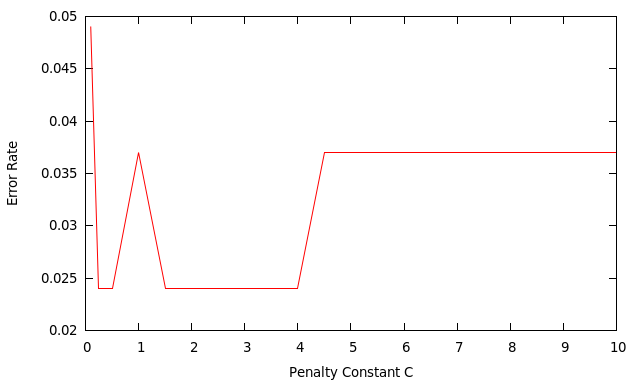
\includegraphics[width=0.9\textwidth]{radial_c_vs_error_rate.png}
\caption{Dual Radial Penality Constant Versus Error Rate}
\end{figure}

\begin{table}\label{table4}
\caption{Dual Radial Digit 3 vs 6 Error}
\begin{center}
\begin{tabular}{llcc}
\toprule
Data Set & Error & \multicolumn{2}{c}{95\% Confidence Interval} \\
\cmidrule(r){3-4}
& & Lower Bound & Upper Bound \\
\midrule
Training & 0.000 & 0.000 & 0.000 \\
Testing & 0.024 & -0.009 & 0.058 \\
\bottomrule
\end{tabular}
\end{center}
\end{table}

Table \ref{table4} indicates that the dual radial SVM classifier perfectly classified the training data set and achieved a \(0.024\) misclassification error rate for the testing data set for digits ''3`` and ''6``. Because the radial kernel performed better than the polynomial kernel, it was chosen for the full problem.

\section{All Digits Radial Kernel}\label{full1}

Because of the size of the full classification problem, the ten hyperplanes (classifying each digit versus all others) were calculated using the NEOS server. The following is an example output from AMPL for the model defining the hyperplane separating digit ''9`` from other digits.

\begin{verbatim}
*************************************************************

   NEOS Server Version 5.0
   Job#     : 328628
   Password : StLZnfpa
   Solver   : nco:LOQO:AMPL
   Start    : 2012-10-20 10:29:39
   End      : 2012-10-20 10:30:39
   Host     : neos-2.chtc.wisc.edu

   Disclaimer:

   This information is provided without any express or
   implied warranty. In particular, there is no warranty
   of any kind concerning the fitness of this
   information  for any particular purpose.
*************************************************************
Job 328628 sent to neos-2.chtc.wisc.edu
password: StLZnfpa
---------- Begin Solver Output -----------
Executing /opt/neos/Drivers/loqo-ampl/loqo-driver.py at time: 2012-10-20 09:29:39.861097
File exists
You are using the solver loqo.

%% YOUR COMMENTS %%%%%%%%%%%%%%%%%%%%%%%
Digit 9
%%%%%%%%%%%%%%%%%%%%%%%%%%%%%%%%%%%%%%%%
Executing AMPL.
processing data.
processing commands.

930 variables, all nonlinear
1 constraint, all linear; 930 nonzeros
	1 equality constraint
1 nonlinear objective; 930 nonzeros.

LOQO 6.07: optimal solution (22 QP iterations, 64 evaluations)
primal objective 252.4800216
  dual objective 252.4800227
a [*] :=
  1 2.71101e-10   234 1.6016e-10    467 2.50501e-10   700 0.359631
  2 3.05019e-10   235 4.45621e-10   468 2.34149e-09   701 3.48449e-10
  3 4.23091e-10   236 2.90327e-10   469 5.3794e-10    702 5.22769e-10
  4 0.109576      237 1.38924e-08   470 1.24123e-08   703 3.31397e-10
  5 4.2032e-10    238 2.45279e-10   471 3.6236e-10    704 0.824905
  6 0.250079      239 3.50097e-10   472 3.74267e-10   705 5.22693e-10
  7 2.30671e-10   240 2.27515e-10   473 2.73113e-10   706 1.11882e-09
  8 2.84478e-10   241 2.17929e-10   474 1.10803e-09   707 3.11901e-10
  9 8.02454e-10   242 1.4388e-10    475 0.239516      708 2.77106e-10
 10 4.44887e-10   243 1.14629e-10   476 1.45518e-10   709 3.80716e-10
 11 4.30417e-10   244 1.95241e-10   477 2.49114e-10   710 1.57364
 12 2.0632e-10    245 0.0438792     478 0.323162      711 0.233815
 13 1.62617e-10   246 4.80989e-10   479 2.43214e-10   712 2
 14 1.85125e-10   247 3.05068e-10   480 2.5741e-08    713 4.41272e-10
 15 3.67808e-10   248 2.37684e-10   481 2.09477e-09   714 7.11917e-10
 16 0.683228      249 2.45333e-10   482 8.60567e-10   715 0.377432
 17 7.60347e-10   250 7.96511e-10   483 4.32497e-10   716 0.789347
 18 6.55803e-10   251 6.06953e-10   484 7.08331e-10   717 4.18937e-10
 19 3.15904e-09   252 1.28136e-10   485 0.379501      718 1.02036e-09
 20 1.79761e-09   253 1.027e-10     486 4.92791e-10   719 5.70864e-10
 21 2.71357e-10   254 1.71695e-10   487 1.97112e-10   720 3.8153e-10
 22 1.92212e-10   255 1.94053e-10   488 3.79737e-10   721 0.102697
 23 4.72529e-10   256 9.73284e-11   489 0.772318      722 2.15089e-10
 24 3.82344e-10   257 1.02502e-10   490 2.1232e-10    723 8.8216e-10
 25 0.381271      258 1.851e-10     491 1.24123e-08   724 1.18103e-09
 26 1.02796       259 1.22668e-10   492 3.79737e-10   725 2
 27 3.1117e-10    260 1.40462e-10   493 2.37014e-10   726 1.22912
 28 6.5167e-10    261 8.83629e-10   494 6.491e-10     727 4.77642e-10
 29 2.82269e-10   262 0.194724      495 3.14507e-10   728 2.59238e-09
 30 2.82269e-10   263 5.0111e-10    496 3.7312e-10    729 5.66192e-10
 31 2.99342e-10   264 1.37391e-10   497 1.72088e-09   730 1.3929
 32 3.23035e-09   265 1.54257e-10   498 2.77638e-10   731 2.61826e-10
 33 1.41332e-09   266 2.17847e-10   499 3.78012e-10   732 2.18425e-10
 34 3.23009e-10   267 2.95835e-10   500 5.56905e-10   733 1.69884e-10
 35 2.09445e-10   268 4.61047e-10   501 4.86469e-10   734 4.56659e-10
 36 1.73911e-10   269 2.63138e-10   502 2.63285e-10   735 0.944744
 37 2.09983e-10   270 1.53048e-10   503 1.48728e-10   736 2.80759e-10
 38 2.32079e-10   271 7.98238e-09   504 1.73291e-10   737 3.14797e-10
 39 2.07256e-10   272 1.73492e-10   505 1.78373e-10   738 2.53804e-10
 40 8.43713e-10   273 1.576e-10     506 4.06374e-10   739 1.91883e-09
 41 6.89633e-10   274 2.34458e-10   507 3.09927e-10   740 3.9635e-10
 42 9.69144e-10   275 1.64343e-09   508 4.45536e-10   741 6.40784e-10
 43 3.69506e-10   276 9.75552e-11   509 0.197104      742 4.50501e-09
 44 8.66321e-10   277 0.907382      510 4.88489e-10   743 5.5969e-10
 45 2.01125e-10   278 1.37777e-10   511 2.21884e-10   744 1.13731e-09
 46 5.41004e-10   279 1.25353e-10   512 2.21087e-10   745 1.62078e-09
 47 3.11712e-10   280 0.193234      513 1.22901e-10   746 2.01263e-10
 48 1.95829e-10   281 1.91158e-10   514 1.55766e-10   747 4.02059e-10
 49 1.89823e-10   282 3.51499e-10   515 3.61952e-10   748 2.07354e-10
 50 9.82374e-10   283 1.15405       516 2.1553e-09    749 2.65487e-10
 51 2.39294e-10   284 1.69181e-10   517 1.25977e-10   750 9.24614e-10
 52 4.31646e-10   285 2.09273e-10   518 3.50938e-10   751 2.93978e-10
 53 1.9124        286 6.55654e-10   519 0.208998      752 1.5972e-10
 54 7.17336e-10   287 1.5245e-10    520 4.3242e-10    753 1.88076
 55 1.49269e-10   288 1.46503e-10   521 0.369471      754 5.04336e-10
 56 6.38842e-10   289 0.350992      522 7.02628e-10   755 2.23063e-10
 57 3.89553e-10   290 1.40585e-09   523 4.32273e-10   756 2.41409e-10
 58 4.61382e-10   291 2.83884e-10   524 1.02083e-09   757 5.97934e-10
 59 1.77933e-10   292 2.76108e-10   525 4.76128e-10   758 4.21131e-10
 60 5.44408e-10   293 2.54383e-10   526 3.24022e-10   759 3.14079e-10
 61 1.3614e-08    294 8.36921e-10   527 2.55657e-10   760 6.49439e-10
 62 3.0292e-10    295 2.37526e-10   528 0.742058      761 3.32288e-10
 63 9.00929e-10   296 2.24922e-10   529 2.81522e-09   762 2.49214e-10
 64 3.78007e-10   297 2.65072e-10   530 0.0863599     763 2
 65 3.81926e-10   298 5.98991e-10   531 2.33055e-10   764 3.55132e-10
 66 2.95786e-10   299 1.6827e-09    532 1.75012e-10   765 4.88949e-10
 67 2.07422e-10   300 7.81238e-10   533 1.04785e-09   766 2.99525e-10
 68 4.74605e-10   301 2.16943e-09   534 1.28889       767 7.30946e-10
 69 6.31043e-10   302 2.5575e-10    535 1.19216e-10   768 2
 70 4.63083e-10   303 3.02784e-10   536 1.01872e-10   769 2.3616e-10
 71 5.25963e-10   304 3.83526e-10   537 0.0964023     770 0.0651233
 72 0.0412337     305 1.74701e-10   538 0.404344      771 5.04336e-10
 73 5.00319e-10   306 7.27789e-09   539 1.32364       772 2.60638e-10
 74 7.64424e-10   307 1.14898e-09   540 4.03003e-10   773 2.30113e-10
 75 4.39496e-10   308 3.83905e-10   541 1.41606e-09   774 3.40443e-10
 76 2.31741e-10   309 6.24217e-10   542 0.0894632     775 0.884928
 77 3.58044e-10   310 2.43296e-10   543 1.04714e-10   776 2
 78 1.53522e-10   311 2.2286e-10    544 2.54567e-09   777 5.39099e-10
 79 3.51581e-10   312 1.3624e-09    545 2.96457e-10   778 7.83687e-10
 80 1.67697e-09   313 0.583467      546 1.21465e-06   779 2
 81 5.5528e-10    314 1.51987e-10   547 2.27372e-10   780 1.66603e-10
 82 2.17089e-10   315 0.291884      548 3.58942e-10   781 8.89186e-10
 83 1.23393e-10   316 2.61786e-10   549 2.65976e-10   782 6.59965e-10
 84 3.82409e-10   317 1.55724       550 3.16478e-10   783 4.17917e-10
 85 2.10487e-10   318 1.60794e-10   551 2.95451e-10   784 3.00264e-09
 86 7.12124e-10   319 1.38595e-10   552 2             785 1.64987
 87 2.67939e-10   320 2.10814e-10   553 1.08237e-06   786 4.09438e-10
 88 8.25426e-10   321 1.72358e-10   554 1.57536e-09   787 2.5676e-10
 89 2.60847e-10   322 4.31069e-10   555 2.79896e-09   788 1.59218e-10
 90 2.80623e-10   323 4.58035e-10   556 1.01182       789 1.11469e-10
 91 3.16352e-10   324 0.30624       557 4.05125e-10   790 0.956321
 92 8.30895e-10   325 3.54335e-10   558 1.76999e-09   791 1.11849e-09
 93 3.49016e-09   326 4.3598e-08    559 1.17275e-10   792 1.32272e-10
 94 4.09806e-10   327 3.53456e-10   560 2.33212e-10   793 1.19048e-10
 95 6.30306e-09   328 1.52819e-10   561 1.8545e-10    794 1.38924e-08
 96 8.97229e-10   329 2.21054e-10   562 2.58824e-10   795 3.72395e-10
 97 2             330 0.149573      563 1.88812e-10   796 3.33326e-09
 98 2             331 6.26937e-10   564 0.439111      797 1.29808e-09
 99 1.93243e-10   332 1.79231e-06   565 1.10441e-10   798 0.27862
100 2.87027e-10   333 4.84215e-10   566 9.34015e-11   799 5.43061e-10
101 2.1588e-10    334 0.430166      567 2.3838e-10    800 1.21607e-09
102 6.4765e-10    335 1.1239e-10    568 1.26357e-10   801 2.47587e-10
103 2.43151e-10   336 4.77828e-10   569 1.69744e-10   802 1.06501
104 1.35969e-08   337 2.88485e-10   570 2.35892e-10   803 7.64902e-10
105 5.40781e-10   338 1.53918       571 1.4653e-10    804 4.52713e-10
106 8.09785e-08   339 4.82422e-10   572 1.39915e-10   805 0.619685
107 8.58717e-10   340 4.79532e-10   573 2.64903e-10   806 1.60583e-09
108 3.2441e-10    341 2             574 0.000147982   807 3.57382e-10
109 1.6473e-09    342 5.88056e-10   575 2             808 2.79121e-10
110 5.40781e-10   343 4.67158e-10   576 1.47561e-09   809 6.75039e-10
111 4.09806e-10   344 1.39345e-09   577 1.42026e-10   810 2.69312e-10
112 7.99613e-10   345 1.44287e-10   578 2.15975e-10   811 1.12605e-09
113 7.50851e-10   346 2.67635e-10   579 1.41372e-10   812 1.66851e-10
114 7.50851e-10   347 2             580 4.24657e-10   813 0.787009
115 5.57267e-09   348 5.692e-08     581 4.944e-10     814 0.64179
116 2.09736e-09   349 4.94336e-10   582 1.42796e-10   815 0.917067
117 9.29859e-10   350 1.80872e-10   583 2.39219e-10   816 2
118 7.13994e-10   351 1.38657e-10   584 3.4967e-10    817 1.00855
119 7.13994e-10   352 1.44715e-10   585 1.71431e-10   818 3.56913e-10
120 4.36425e-10   353 1.45343e-10   586 1.32596e-10   819 6.34792e-10
121 4.09806e-10   354 2.22983e-10   587 1.1584e-10    820 5.52621e-10
122 4.09806e-10   355 3.69496e-10   588 1.24087e-10   821 2.26768e-10
123 4.36425e-10   356 8.09143e-09   589 1.56414e-10   822 1.84101e-10
124 5.40781e-10   357 1.60399e-10   590 1.45494e-10   823 4.86208e-09
125 1.25295e-09   358 2.57085e-10   591 1.32502e-10   824 6.17232e-10
126 1.9078e-09    359 4.77983e-10   592 1.9904e-10    825 2.8522e-10
127 2.08638e-09   360 1.95812e-09   593 1.75483e-10   826 1.81175e-10
128 9.37852e-10   361 0.106277      594 4.54888e-10   827 1.33675e-05
129 1.9085e-10    362 0.0269783     595 1.86434e-10   828 3.62899e-09
130 1.95002e-10   363 2             596 1.63018e-10   829 3.06503e-10
131 3.0967e-09    364 4.93556e-10   597 2.5987e-10    830 3.16941e-10
132 2.66968e-10   365 9.04538e-09   598 1.10441e-10   831 5.7169e-10
133 5.40781e-10   366 2             599 1.83984e-10   832 3.73125e-10
134 8.12617e-10   367 1.59059e-09   600 2.10587e-10   833 4.98156e-10
135 1.52128e-10   368 0.228184      601 1.32576e-09   834 1.44482e-10
136 1.62219e-10   369 1.77301e-10   602 2.17434e-10   835 1.86059e-10
137 1.83919       370 3.48994e-10   603 1.59152e-10   836 2
138 3.22273e-09   371 2.37236e-10   604 1.64217e-10   837 4.0558e-09
139 4.91619e-10   372 3.44807e-10   605 2.30663e-10   838 2
140 2.36073e-10   373 1.38252       606 1.28726e-10   839 2
141 0.946182      374 4.21276e-09   607 9.87904e-11   840 2
142 1.66133e-10   375 1.9692e-10    608 4.01117e-10   841 2
143 5.40781e-10   376 5.74977e-10   609 1.64898e-09   842 2
144 3.88946e-10   377 4.52498e-10   610 1.45439e-10   843 2
145 8.36234e-10   378 2             611 2.27339e-10   844 2
146 8.36234e-10   379 1.69934e-10   612 9.31009e-11   845 2
147 0.17706       380 0.155851      613 1.33547e-10   846 2
148 1.7411e-10    381 7.34285e-10   614 1.40848e-10   847 2
149 0.516598      382 1.85444e-10   615 1.75352e-10   848 2
150 2.18358e-09   383 0.745732      616 1.86419e-10   849 2
151 1.7936e-09    384 1.49196e-10   617 1.49942e-10   850 2
152 5.19966e-09   385 8.86431e-10   618 2.47291e-10   851 2
153 7.13994e-10   386 2             619 2.0376e-10    852 2
154 7.02989e-10   387 1.7429        620 2.5104e-10    853 2
155 3.1706e-10    388 2             621 1.90586e-10   854 2
156 2.52862e-10   389 2             622 2.1558e-10    855 2
157 4.36425e-10   390 2             623 1.66266e-10   856 1.85007
158 4.36425e-10   391 2             624 1.52159e-10   857 1.89927e-10
159 9.77376e-10   392 1.77226       625 1.7842e-10    858 2
160 7.23251e-10   393 2             626 1.5398e-10    859 2
161 1.2839        394 2             627 1.91512e-10   860 2
162 2.60063e-10   395 1.15625e-09   628 1.37507e-10   861 2
163 2             396 2.5941e-09    629 1.30145e-10   862 2
164 2.52862e-10   397 2.21047e-10   630 8.61982e-10   863 2
165 6.16682e-10   398 3.26363e-10   631 1.9822e-09    864 2
166 1.74931e-10   399 6.09761e-10   632 1.37434e-10   865 2
167 2.01293e-10   400 1.29194e-09   633 1.22209e-10   866 2
168 3.05005e-10   401 2.5021e-10    634 1.5289e-09    867 2
169 1.4835        402 1.14897       635 7.19225e-10   868 2
170 4.99702e-10   403 2             636 1.11619e-10   869 1.18827
171 8.06624e-10   404 0.470773      637 5.08321e-10   870 3.47457e-10
172 4.62761e-10   405 0.470813      638 1.83445e-10   871 2
173 5.40781e-10   406 2             639 1.03108e-10   872 2
174 5.40781e-10   407 2             640 3.65087e-10   873 2
175 2.52862e-10   408 7.40393e-09   641 1.58791e-10   874 2
176 2.6558e-10    409 0.29403       642 1.44478e-10   875 1.57489e-09
177 3.89793e-10   410 1.77251       643 2.32835e-10   876 2
178 5.4632e-10    411 2             644 1.40123e-10   877 1.83278
179 2.42753e-10   412 2.03853e-09   645 9.91711e-11   878 5.98553e-10
180 2.00929e-10   413 2.97271e-10   646 2.38138e-10   879 2
181 2.52862e-10   414 2             647 1.90311e-10   880 2
182 4.09806e-10   415 1.34852       648 1.4179e-10    881 2
183 2.40431e-09   416 2             649 1.24351e-10   882 2
184 4.09806e-10   417 2             650 5.47807e-10   883 0.977972
185 5.40781e-10   418 2             651 1.74586e-10   884 1.41135
186 1.35969e-08   419 2             652 1.0955e-09    885 2
187 1.95928e-10   420 0.838651      653 3.7282e-10    886 2
188 1.49141e-10   421 2             654 0.594143      887 2
189 2.24096e-10   422 2.51289e-10   655 4.74707e-10   888 2
190 1.30161e-10   423 3.52869e-10   656 2.93693e-10   889 2
191 2.0539e-10    424 1.76969e-10   657 3.84425e-10   890 2
192 1.79612e-10   425 0.803506      658 2.77683e-10   891 2
193 2.80625e-10   426 2             659 7.22721e-10   892 2
194 1.48551e-10   427 0.722357      660 2.1289e-09    893 2
195 1.26908e-10   428 2.65739e-10   661 4.38202e-10   894 2
196 4.02715e-10   429 2.34939e-10   662 0.930195      895 2
197 1.91448e-10   430 1.23701e-08   663 4.2839e-10    896 1.40009
198 8.49145e-10   431 6.42203e-09   664 1.83399       897 2
199 4.1475e-10    432 1.46948e-09   665 0.716967      898 2
200 1.12113e-09   433 3.68595e-10   666 1.57683       899 2
201 3.26518e-10   434 1.49296e-10   667 2             900 2
202 2.38173e-10   435 1.33733e-10   668 2.2164e-08    901 2
203 3.19017e-10   436 1.9061e-10    669 9.83384e-10   902 2
204 4.76498e-10   437 1.85717e-10   670 5.51473e-10   903 2
205 2.52144e-10   438 7.3294e-09    671 1.5994        904 2
206 3.20552e-10   439 0.504093      672 5.54456e-10   905 2
207 1.36404e-09   440 9.47947e-10   673 4.26644e-10   906 2
208 2.40734e-10   441 1.83519e-10   674 8.5777e-10    907 2
209 1.57952e-10   442 2             675 2.15896e-10   908 2
210 1.22189e-10   443 5.05152e-10   676 3.16582e-10   909 2
211 8.83539e-10   444 2             677 1.9067e-10    910 2
212 1.41483e-10   445 2             678 2.2583e-10    911 1.64253
213 1.41631e-09   446 2             679 1.62111e-08   912 2
214 2.87328e-10   447 2             680 4.07298e-10   913 2
215 5.71811e-10   448 1.8435        681 2.19933e-06   914 0.178782
216 6.97345e-10   449 7.58958e-10   682 4.0436e-10    915 2
217 5.42887e-10   450 8.69382e-11   683 4.47194e-10   916 2
218 9.38976e-11   451 4.5594e-10    684 4.2523e-10    917 2
219 2.38589e-10   452 2             685 1.64681       918 0.000627353
220 3.25799e-10   453 8.20168e-10   686 0.839054      919 2
221 1.547e-10     454 2.24785e-10   687 3.65933e-09   920 2
222 2.7325e-10    455 1.69306e-10   688 2.91171e-10   921 2
223 2.55517e-10   456 1.67446e-09   689 5.33593e-10   922 2
224 4.17518e-10   457 2             690 2             923 2
225 4.42715e-10   458 1.67866e-10   691 5.28966e-10   924 2
226 1.84776e-10   459 1.7413e-10    692 3.81113e-10   925 2
227 1.21656e-10   460 1.6457        693 3.88723e-10   926 2
228 1.969e-10     461 2             694 3.17057e-10   927 2
229 1.32151e-10   462 3.32011e-10   695 4.07349e-10   928 8.44138e-10
230 1.71673e-10   463 2.65239e-09   696 2.36066e-10   929 1.09846e-09
231 2.24904e-10   464 4.55434e-10   697 1.51219       930 2
232 2.53547e-10   465 1.7445e-10    698 0.299297
233 3.77923e-09   466 4.01709e-10   699 3.61046e-10
;

\end{verbatim}

The above results contain 102 support vectors from among the 930 input data elements. This relatively low percentage of the total input data elements suggests that the choice of \(C=2\) was a reasonable one. Calculating the \(b\) value for each support vectors verifies that we get the same value for each.

\begin{verbatim}

#alpha index, alpha value, calculated b
3 0.1096 1.652528615299
5 0.2501 1.652529353414
15 0.6832 1.652531306182
24 0.3813 1.652527500127
25 1.0280 1.652530795828
52 1.9124 1.652527383484
71 0.0412 1.652528013565
136 1.8392 1.652532499353
140 0.9462 1.652528563888
146 0.1771 1.652527764148
148 0.5166 1.652527893505
160 1.2839 1.652530132401
168 1.4835 1.652529075643
244 0.0439 1.652531164695
261 0.1947 1.652530083805
276 0.9074 1.652526149271
279 0.1932 1.652528417878
282 1.1541 1.652524420840
288 0.3510 1.652529477347
312 0.5835 1.652528225378
314 0.2919 1.652528039180
316 1.5572 1.652526531397
323 0.3062 1.652529164868
329 0.1496 1.652529910410
333 0.4302 1.652529765260
337 1.5392 1.652531061831
360 0.1063 1.652530379536
361 0.0270 1.652530174674
367 0.2282 1.652530070206
372 1.3825 1.652528458326
379 0.1559 1.652526904421
382 0.7457 1.652529520710
386 1.7429 1.652530637204
391 1.7723 1.652527386907
401 1.1490 1.652524444029
403 0.4708 1.652528387177
404 0.4708 1.652528387177
408 0.2940 1.652528368235
409 1.7725 1.652527020817
414 1.3485 1.652523632212
419 0.8387 1.652528711269
424 0.8035 1.652526733254
426 0.7224 1.652529242901
438 0.5041 1.652528431643
447 1.8435 1.652527445195
459 1.6457 1.652525583912
474 0.2395 1.652528624423
477 0.3232 1.652527227243
484 0.3795 1.652528412434
488 0.7723 1.652526536987
508 0.1971 1.652529961663
518 0.2090 1.652526358944
520 0.3695 1.652531027114
527 0.7421 1.652528796724
529 0.0864 1.652528840065
533 1.2889 1.652528843938
536 0.0964 1.652528090385
537 0.4043 1.652527522760
538 1.3236 1.652526943084
541 0.0895 1.652530441145
555 1.0118 1.652528984266
563 0.4391 1.652531006415
653 0.5941 1.652528068457
661 0.9302 1.652527391766
663 1.8340 1.652524944961
664 0.7170 1.652530665392
665 1.5768 1.652526744789
670 1.5994 1.652524876784
684 1.6468 1.652526021447
685 0.8391 1.652526918713
696 1.5122 1.652527315814
697 0.2993 1.652529869617
699 0.3596 1.652529917065
703 0.8249 1.652525043714
709 1.5736 1.652525375261
710 0.2338 1.652527238423
714 0.3774 1.652526221993
715 0.7893 1.652527541293
720 0.1027 1.652525252885
725 1.2291 1.652527538439
729 1.3929 1.652531032958
734 0.9447 1.652526378642
752 1.8808 1.652529939311
769 0.0651 1.652524700601
774 0.8849 1.652528444583
784 1.6499 1.652527632173
789 0.9563 1.652530350245
797 0.2786 1.652526661335
801 1.0650 1.652523415984
804 0.6197 1.652528203919
812 0.7870 1.652527593202
813 0.6418 1.652528426022
814 0.9171 1.652528377663
816 1.0086 1.652526486404
855 1.8501 1.652526793776
868 1.1883 1.652533655177
876 1.8328 1.652531890671
882 0.9780 1.652531290116
883 1.4114 1.652532387564
895 1.4001 1.652525486924
910 1.6425 1.652530782561
913 0.1788 1.652525697648

\end{verbatim}

\begin{table}\label{tablefull}
\caption{Dual Radial All Digits Error}
\begin{center}
\begin{tabular}{llcc}
\toprule
Data Set & Error & \multicolumn{2}{c}{95\% Confidence Interval} \\
\cmidrule(r){3-4}
& & Lower Bound & Upper Bound \\
\midrule
Training & 0.053 & 0.038 & 0.067 \\
Testing & 0.222 & 0.182 & 0.262 \\
\bottomrule
\end{tabular}
\end{center}
\end{table}

As indicated in Table \ref{tablefull}, the overall testing misclassification error achieved by the radial SVM classifier was \(0.222\). This is significantly better than the \(0.9\) misclassification error that we would expect to achieve by random guessing.

\end{document}
